
\chapter{Einleitung}
\thispagestyle{fancy}

\iffalse
\begin{quote}
This year’s Nobel Laureates are rewarded for having invented a new energy-efficient and environment-friendly light source – the blue light-emitting diode (LED). In the spirit of Alfred Nobel the Prize rewards an invention of greatest benefit to mankind; using blue LEDs, white Light can be created in a new way. \cite{nobelp} \end{quote}
\noindent
Dieser Satz, den die Schwedische Akademie der Wissenschaft nach der Vergabe des Nobelpreises an die Entwicklung der blauen LED (kurz, light emitting diode) im Jahr 2014 an die Presse veröffentlichte, fasst treffend zusammen, wie hoch die Bedeutung der auf Halbleiterkristallen basierenden optischen Bauelemente ist \cite{kneissl}. 

\fi

LEDs nehmen einen fundamentalen und immer bedeutender werdenden Teil unseres alltäglichen Lebens ein. Ausgezeichnet durch ihre hervorragende Effizienz, konkurrenzlosen Lebensdauer und geringen Dimension übernimmt sie durch eine immer höher werdende Lichtausbeute zusehends neue Anwendungsbereiche.
\newline
Insbesondere auf Galliumnitrid (GaN) basierende Halbleitermaterialien haben einen bahnbrechenden Weg hingelegt, der zur Entwicklung von hoch effizienten und leuchtstarken blauen LEDs führte und ebenfalls Grundlage für die Entwicklung in andere hochenergetische Wellenlängenbereiche darstellt \cite{risk} \cite{Shuji1999CandelaclassHI} \cite{10007979421}. So ebnet GaN auch den Weg für die Erzeugung von ultraviolett emittierenden Leuchtdioden. Der ultraviolette Spektralbereich, der sich in den UV-A (400 nm bis 320 nm), UV-B (320 nm bis 280) und UV-C Bereich (280 nm bis 200 nm) unterteilt, ist bedeutend für eine sehr hohe Anzahl spezieller Anwendungsbereiche. 
\newline
Beispielsweise bieten sich UV-LEDs an, um die bisher für Wasseraufbereitung genutzten Quecksilberdampflampen zu ersetzen \cite{Vilhunen2009} \cite{WURTELE20111481}. Bislang werden für deren Betrieb Hochspannungsnetzteile verwendet, die einen mobilen Einsatz erheblich erschweren können. Hier bietet sich die Möglichkeit Abhilfe durch UV-LEDs zu verschaffen, da diese durch ihr kleines Format und durch die niedrigen Betriebsspannungen einen mobilen Einsatz ermöglichen. Ein weiteres Anwendungsgebiet ist die industrielle Aushärtung/Aufbrechung von Lacken und die Gasdetektion \cite{0268-1242-26-1-014036} \cite{LALINSKY2010152}. 
\iffalse
\begin{figure}[htb]
    \centering
    \begin{minipage}[t]{0.49\linewidth}
        \centering
        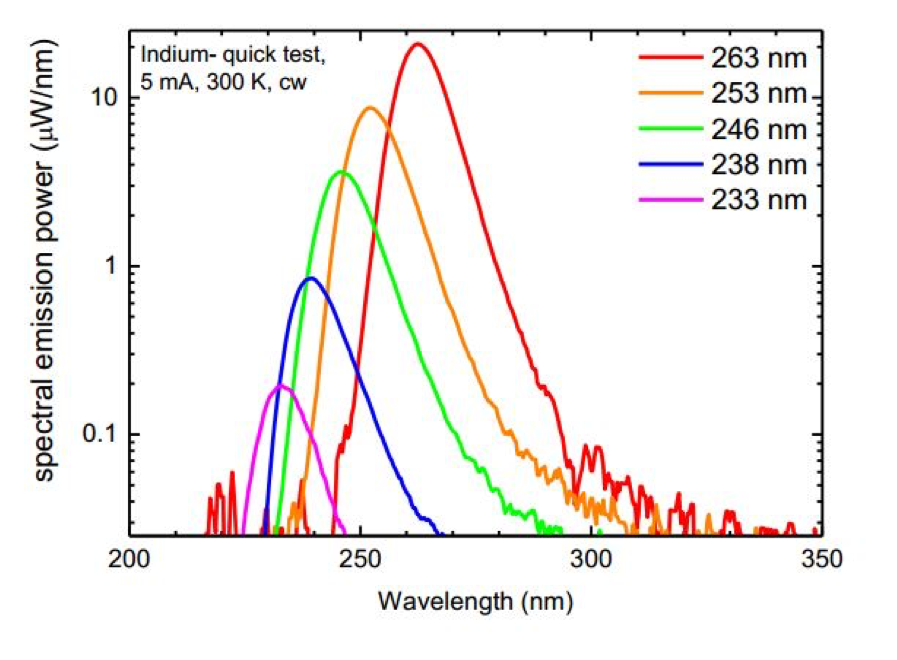
\includegraphics[width=\linewidth]{Bilder/SpectralEmissionPower_Wavelength.png}
        \caption{Spektrale Emissionsleistung für 5 verschiedene Wellenlängen von 263 nm bis 233 nm. Die Grafik zeigt, dass die spektrale Emissionsleistung mit sinkender Wellenlänge ebenfalls sinkt\cite{semreich}.}
        \label{fig:specPowWVL}
    \end{minipage}
    \hfill
    \begin{minipage}[t]{0.49\linewidth}
        \centering
        \includegraphics[width=\linewidth]{Bilder/Schichten.png}
        \caption{Aufbau einer LED-Heterostruktur mit vielen Schichten die unterschiedlichen Zwecken dienen.}
        \label{fig:schichtenLED}
    \end{minipage}
\end{figure}
\noindent
%
\fi
\newline
Für alle diese Anwendungsbereiche ist eine hohe Ausgangsleistung notwendig. Allerdings sind die spektrale Emissionsleistung mit kleiner werdenden Wellenlängen signifikant \cite{0268-1242-26-1-014036}. Der Grund dafür ist, dass UV-LEDs bisher einer geringen Effizienz unterliegen, die quantitativ als Externe Quanteneffizienz (EQE) ausgedrückt wird und sich aus dem Produkt der internen Quanteneffizenz (IQE), Extraktionseffizenz (EE) und Injektionseffizienz (INJ) zusammensetzt.
\iffalse
%
\begin{equation}
    EQE = IQE \cdot EE \cdot INJ
\end{equation}
%
\fi
\newline
Die Gründe für die geringe Effizienz sind vielfältig. LEDs bestehen aus einer Vielzahl an Schichten, die unterschiedlichen Funktionen dienen. Diese Schichten werden auf Substraten aufgewachsen. Eine hohe Substratqualität ist also der Grundbaustein für die optischen Eigenschaften und damit besonders entscheidend. Denn eine geringe Defektdichte im Substrat geht einher mit einer ebenfalls geringen Defektdichte in den aufgewachsenen Schichten und damit insbesondere der aktiven Zone, in der Elektronen und Löcher rekombinieren und Licht emittiert wird.
\newline
Ein weiteres Problem im Zusammenhang mit den geringen Defektdichten ist ein Mangel an geeigneten Substratmaterialien. So wird aufgrund des Mangels an AlN-Substraten, beruhend auf den Preis der Herstellung, auf Saphir Substrate ausgewichen. Diese sind im fernen UV transparent und zusätzlich in großen Mengen in guter Qualität herstellbar. Problematisch jedoch ist die hohe Gitterfehlanpassung durch die relativ großen Unterschiede zwischen den Gitterkonstanten von AlN/GaN und Saphir. Durch diese sind AlN- und AlGaN-Schichten nicht vollverspannt aufwachsbar. Das führt dazu, dass die Schichten relaxieren, weil die Elastizität der Schicht nicht groß genug im Vergleich zur Verspannungsenergie ist. Die Relaxation führt zur Entstehung von Versetzungen und Rissen. Die Versetzungen agieren im Kristall als sogenannte nicht-strahlende Rekombinationszentren, welche die IQE verringern. 
\newline
Die Hauptthematik dieser Arbeit liegt in der Bestimmung der IQE von AlGaN - Heterostrukturen mit hohem Al-Gehalt mit Hilfe von temperatur- und leistungsdichteabhängigen Photolumineszenzmessungen.
Daher wird im ersten Teil dieser Arbeit auf die grundlegenden Schwierigkeiten bei der Bestimmung der IQE durch temperaturabhängige Photolumineszenzmessungen eingegangen und das bisher verwendete Modell angepasst. 
\newline
Mit dieser Anpassung widmet sich diese Arbeit dann der Untersuchung von AlGaN-MQWs in UVC-LED-Heterostrukturen mit variierenden Quantentopf(eng.: quantum well, kurz: QW)-Dicken mit dotierten und undotierten Barrieren. Mit Hilfe von temperatur- und leistungsdichteabhängiger UV-Photolumineszenz(kurz.: PL) wird der Einfluss der variierenden QW-Dicke und Dotierung auf die interne Quanteneffizienz und die Emissionsenergien untersucht. Ziel ist es ein optimales Design und damit ein optimiertes Verhältnis zwischen Abschirmung des Quantum Confined Stark Effect (QCSE) und Ladungsträgereinschluss für die MQW-Heterostruktur zu bestimmen.
\newline
Als nächstes wird dann wird der Einfluss des Fehlschnittwinkels des Substrates und der Nutzung eines Übergitters auf die IQE von AlGaN-Heterostrukturen von UVC-Laserdioden(kurz.: LD) untersucht. Der Fehlschnittwinkel nimmt deutlichen Einfluss auf die Wachstumskinetik und somit auf die Anordnung der monoatomaren Schichten. So können sie zum Abknicken von Versetzungen führen und damit zu einer insgesamt reduzierten Versetzungsdichte \cite{jeschke}. Die Nutzung eines Übergitters erlaubt ein sogenanntes Verspannungs-Managment, mit dem ebenfalls eine deutliche Verringerung der Versetzungsdichte zu erreichen ist \cite{doi:10.1063/1.2136424}. Der Einfluss des Übergitters und des Fehlschnittwinkels sollten somit an der PL-IQE zu erkennen sein. Insbesondere aber auch an der Oberflächenmorphologie auf die zusätzlich mit Hilfe von Kathodolumineszenzspektroskopie (engl. cathodoluminescence, CL) und Rasterkraftmikroskopie (engl. atomic force microscopy, AFM) eingegangen wird.
\newline
Darauf folgt die Überprüfung theoretischer Simulationen der Polarisation für AlGaN-UVC-Heterostrukturen mit Hilfe von Photolumineszenzmessungen. Die Polarisation hat bedeutenden Einfluss auf die Extraktionseffizienz (EE) und somit auf die EQE.
\newline
Zuletzt wird eine Methode analysiert und versucht anzuwenden, die eine Möglichkeit beschreibt, durch leistungsdichteabhängige Messungen bei Raumtemperatur die IQE zu bestimmen. Das ist insofern ein Vorteil, dass ein aufwendiges Runterkühlen auf Tieftemperatur($5 \thinspace K$) nicht notwendig ist und daneben auch die Basis für einen Vergleich mit der temperaturabhängigen Standardmethode liefert.













